\chapter{Results and Observations}

This chapter presents the experimental results obtained from implementing Zero-Knowledge Logistic Regression using the GNARK framework. Analysis was done for proof sizes, performance, scalability, batch processing efficiency, and security validation. All experiments were conducted on a fixed dataset of 500 student records with varying batch sizes ranging from 5 to 100 samples per proof to determine the optimal batching strategy.

\section{Proof Size Analysis}

The PLONK proof system demonstrates constant proof size regardless of the circuit complexity or number of samples processed. 

\begin{figure}[h]
    \centering
    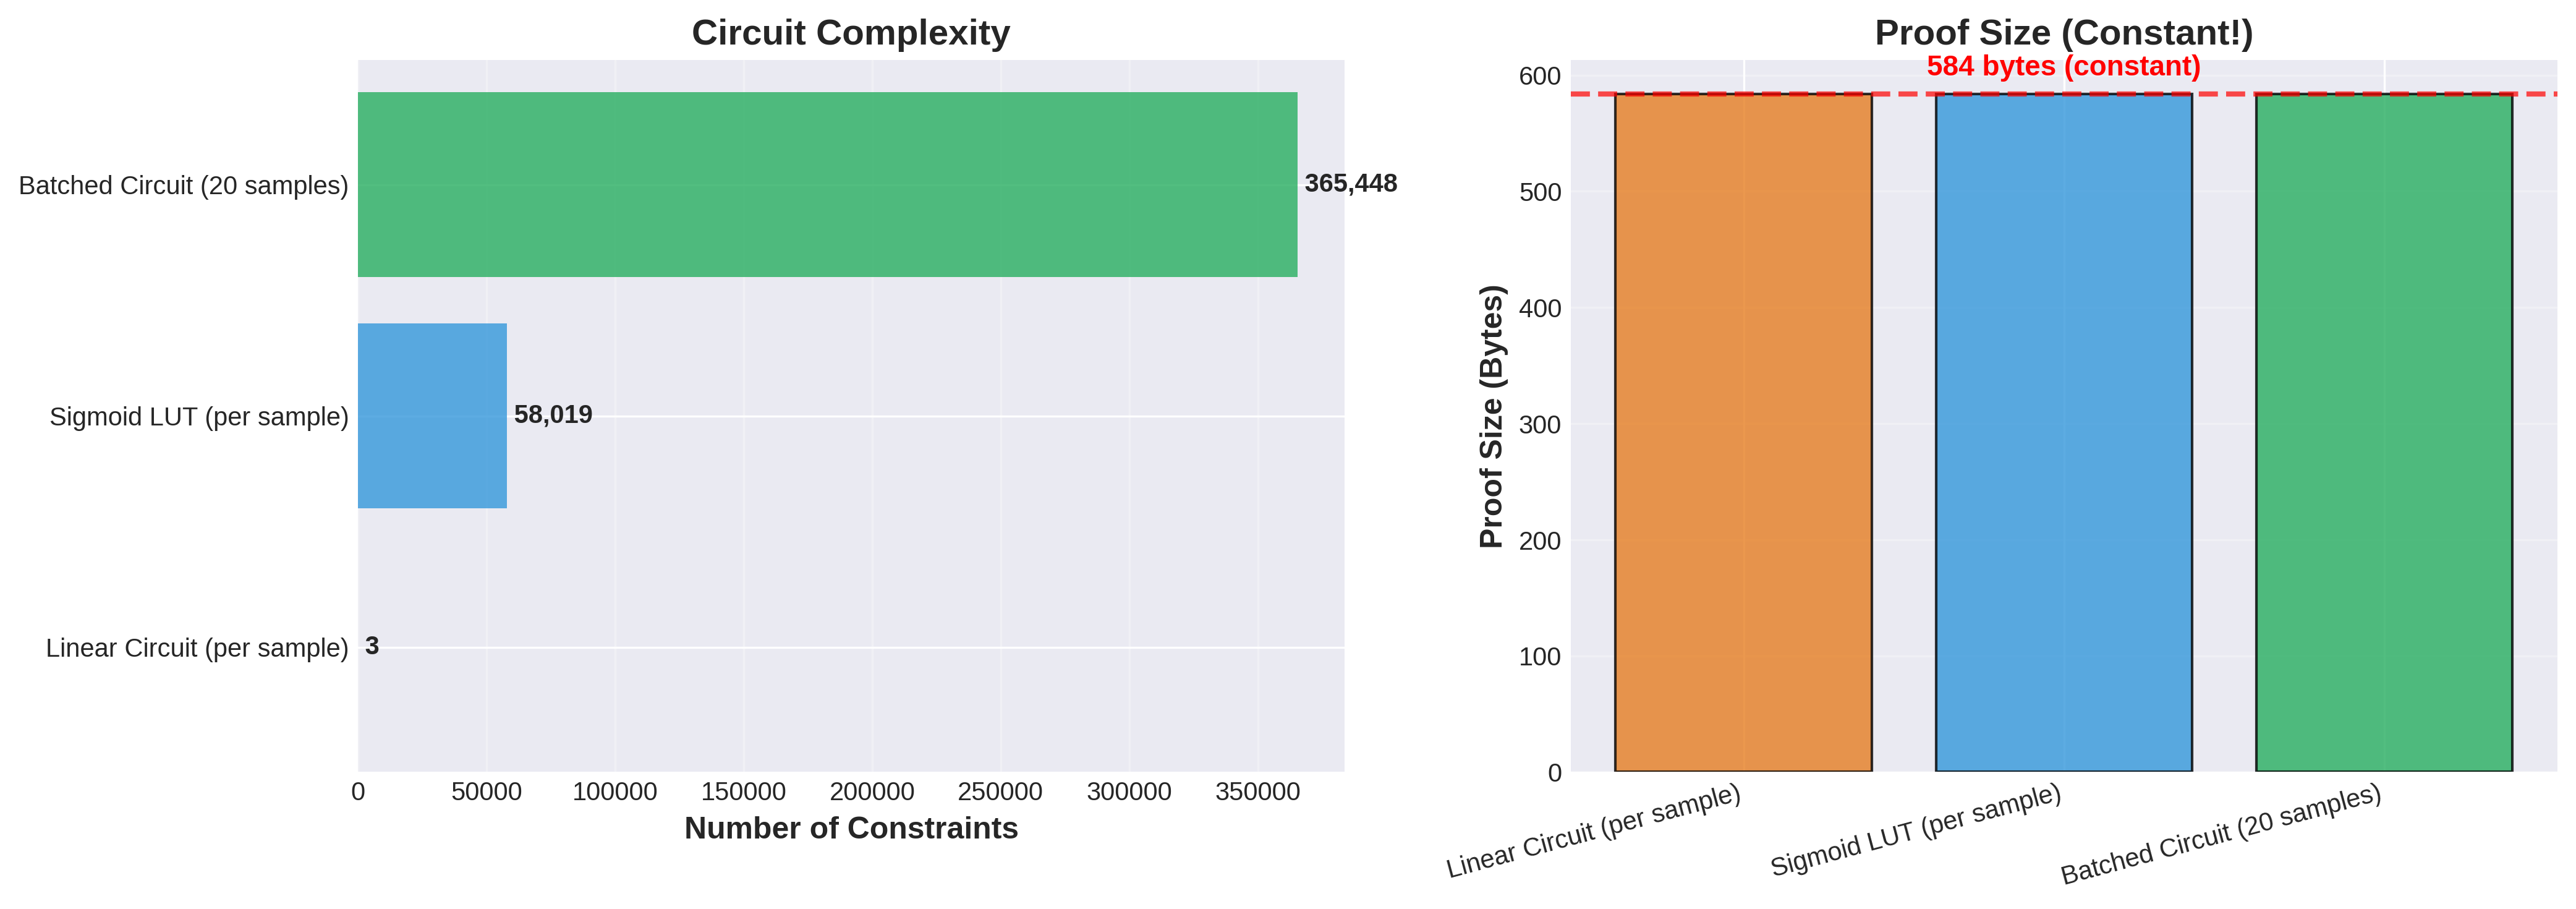
\includegraphics[width=0.8\textwidth]{proof_size_comparison.png}
    \caption{Constant proof size confirms succinctness of PLONK}
    \label{fig:proof_size_comparison}
\end{figure}

As shown in Figure~\ref{fig:proof_size_comparison}, both circuit implementations, individual samples and batched samples, generate proofs of exactly 584 bytes. The circuit for individual samples contains 58,028 constraints, whereas the batched version contains 365,448 constraints, yet both produce proofs of identical size. This constant proof size confirms PLONK's succinctness property, where the proof size depends only on the security parameter and not on the circuit complexity. The communication cost therefore remains minimal, regardless of the computation complexity being verified.

\section{Batch Size Optimization Analysis}

The selection of optimal batch size requires careful analysis of the trade-off between circuit complexity and proof generation overhead. Experiments were conducted with batch sizes of 5, 10, 20, 25, 50, and 100 samples per proof on a fixed dataset of 500 samples.

\begin{figure}[h]
    \centering
    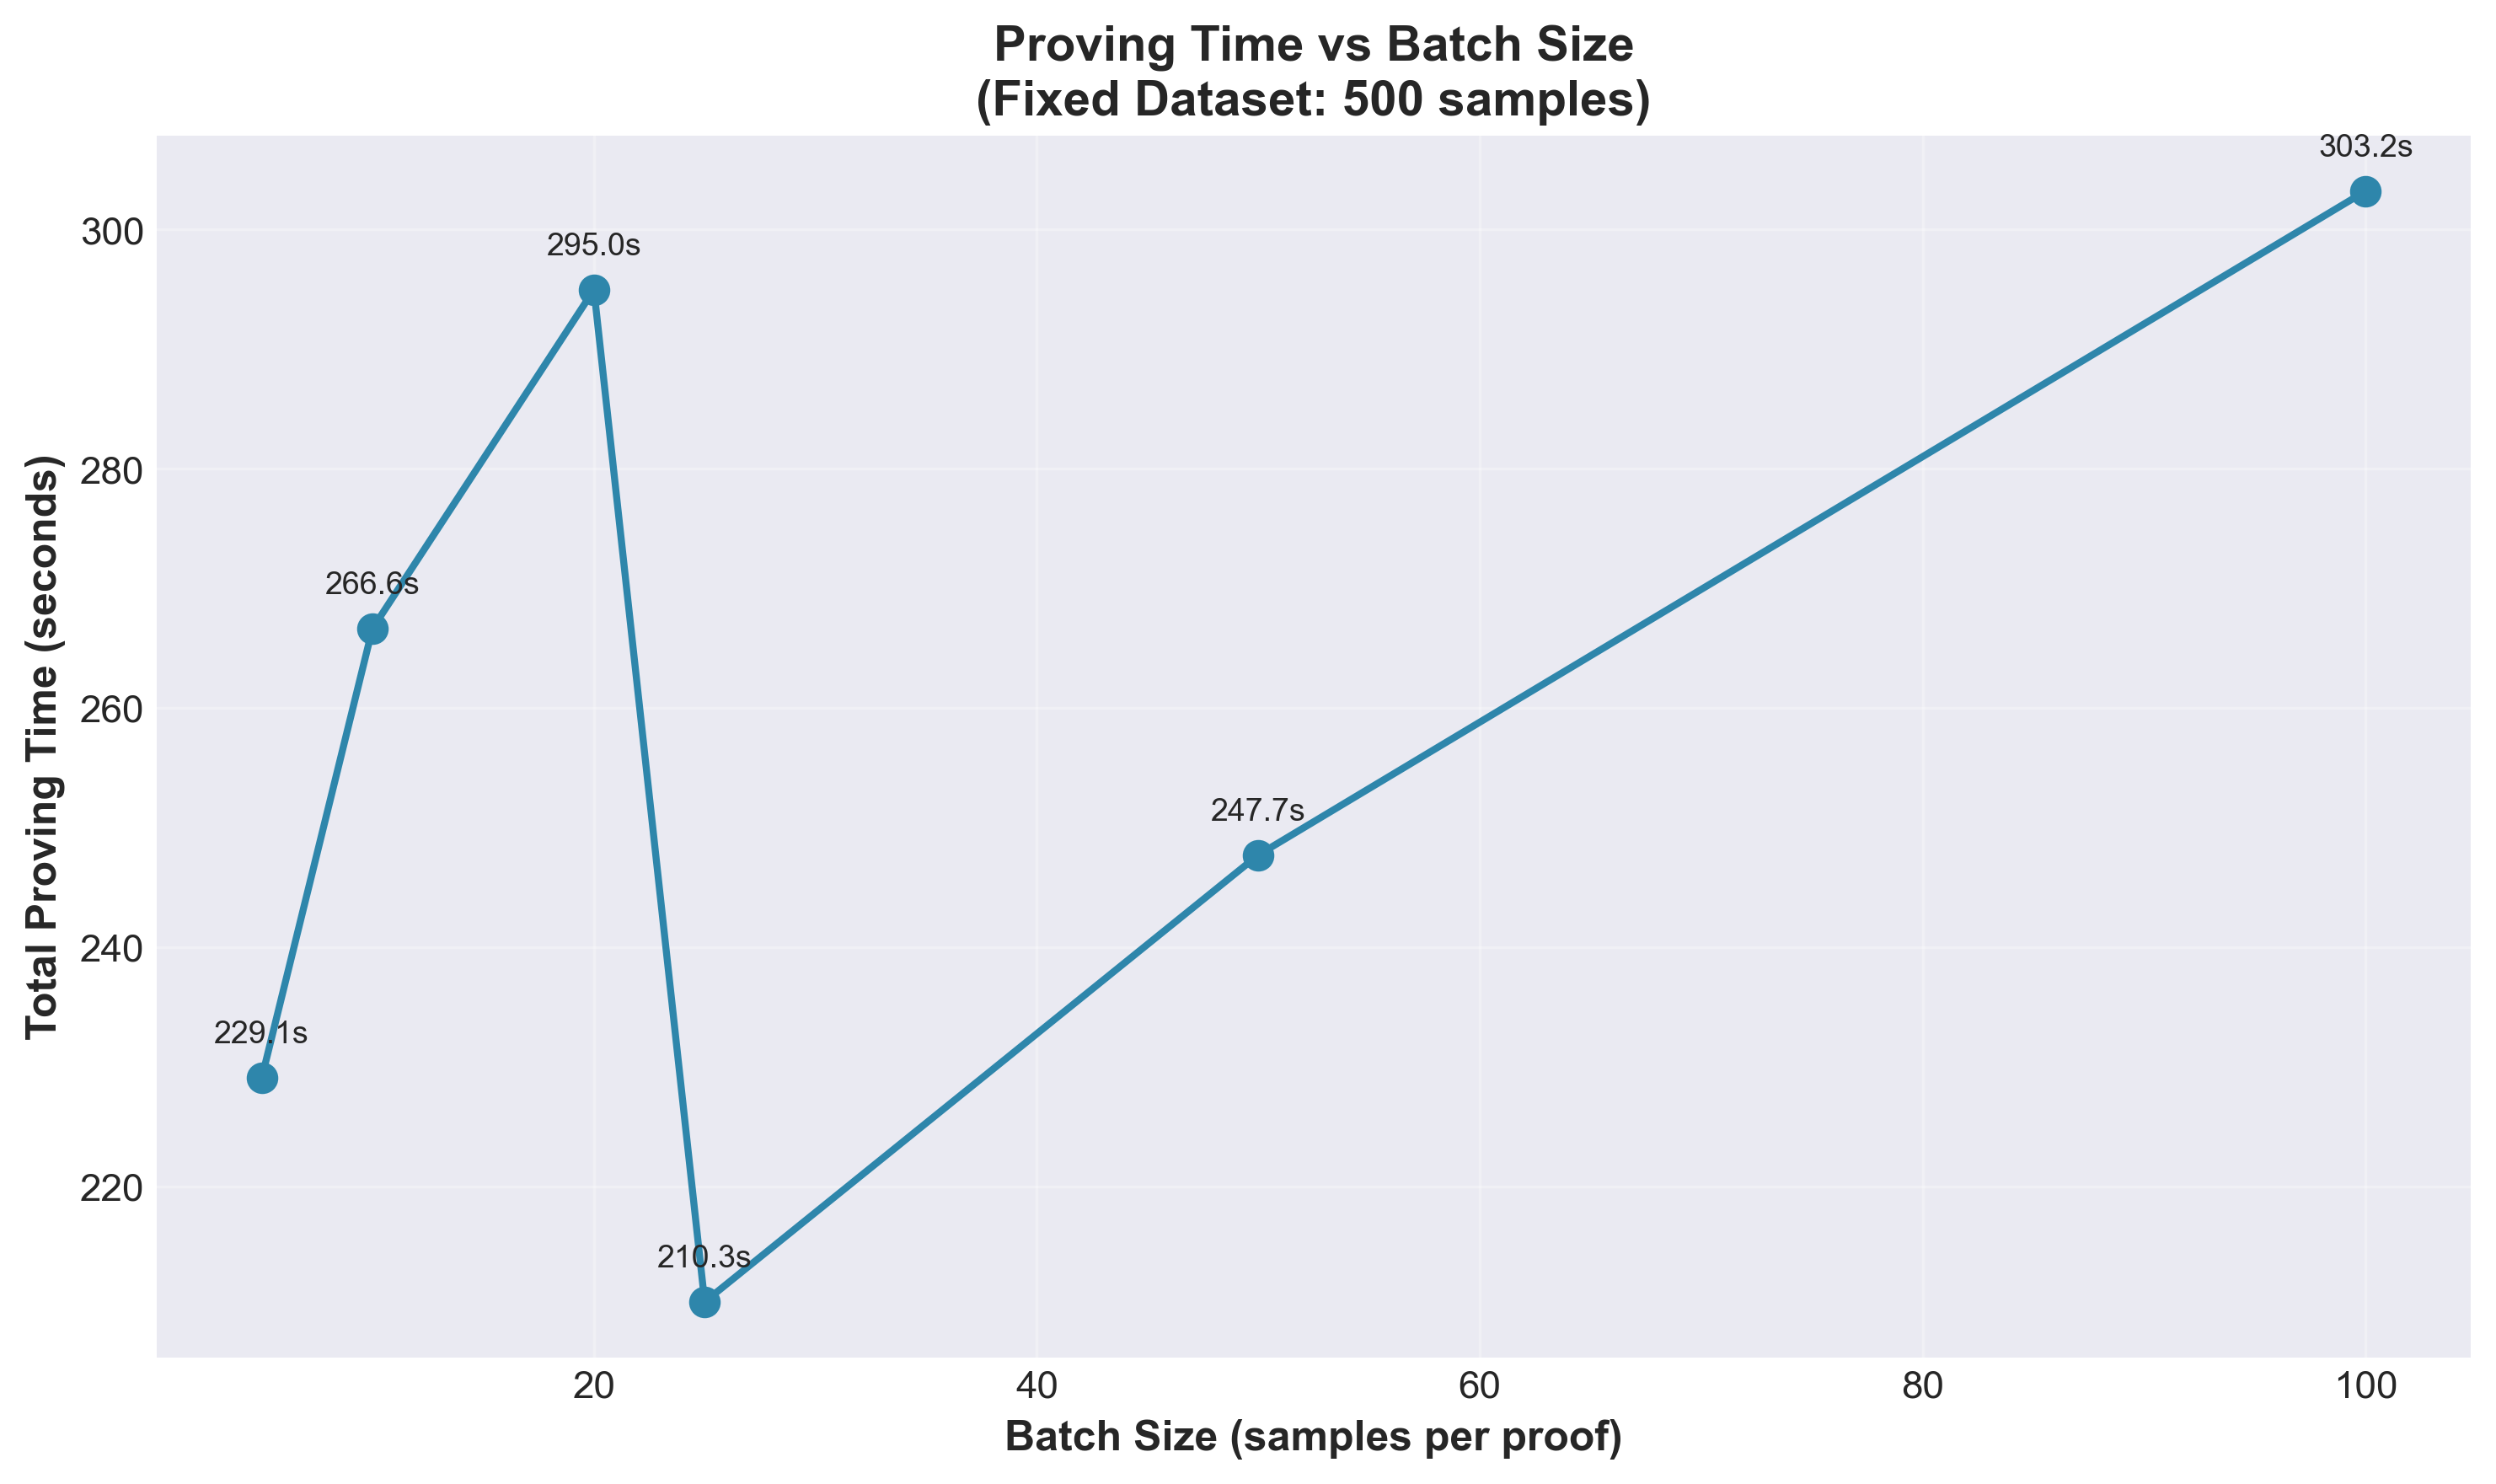
\includegraphics[width=0.8\textwidth]{batch_proving_time.png}
    \caption{Total proving time exhibits non-monotonic behavior across batch sizes}
    \label{fig:batch_proving_time}
\end{figure}

Figure~\ref{fig:batch_proving_time} reveals a critical finding that challenges the intuition that larger batches always improve performance. The proving time initially increases from 229 seconds at batch size 5 to a peak of 295 seconds at batch size 10, then drops sharply to 210 seconds at batch size 25 before rising again to 303 seconds at batch size 100. This non-monotonic behavior indicates that batch size 25 represents a local optimum where the circuit compilation and constraint satisfaction mechanisms achieve maximum efficiency. The sharp increase from batch size 5 to 10 suggests that small batches incur disproportionate overhead in circuit setup, while the subsequent decrease to batch size 25 demonstrates improved amortization of shared computation. Beyond batch size 25, the proving time increases linearly as circuit complexity dominates, with each additional sample contributing proportionally more constraints that offset the benefits of batching.

\section{Throughput Characteristics}

System throughput measures the rate at which samples can be processed, proved and verified, accounting for both proving and verification overhead.

\begin{figure}[h]
    \centering
    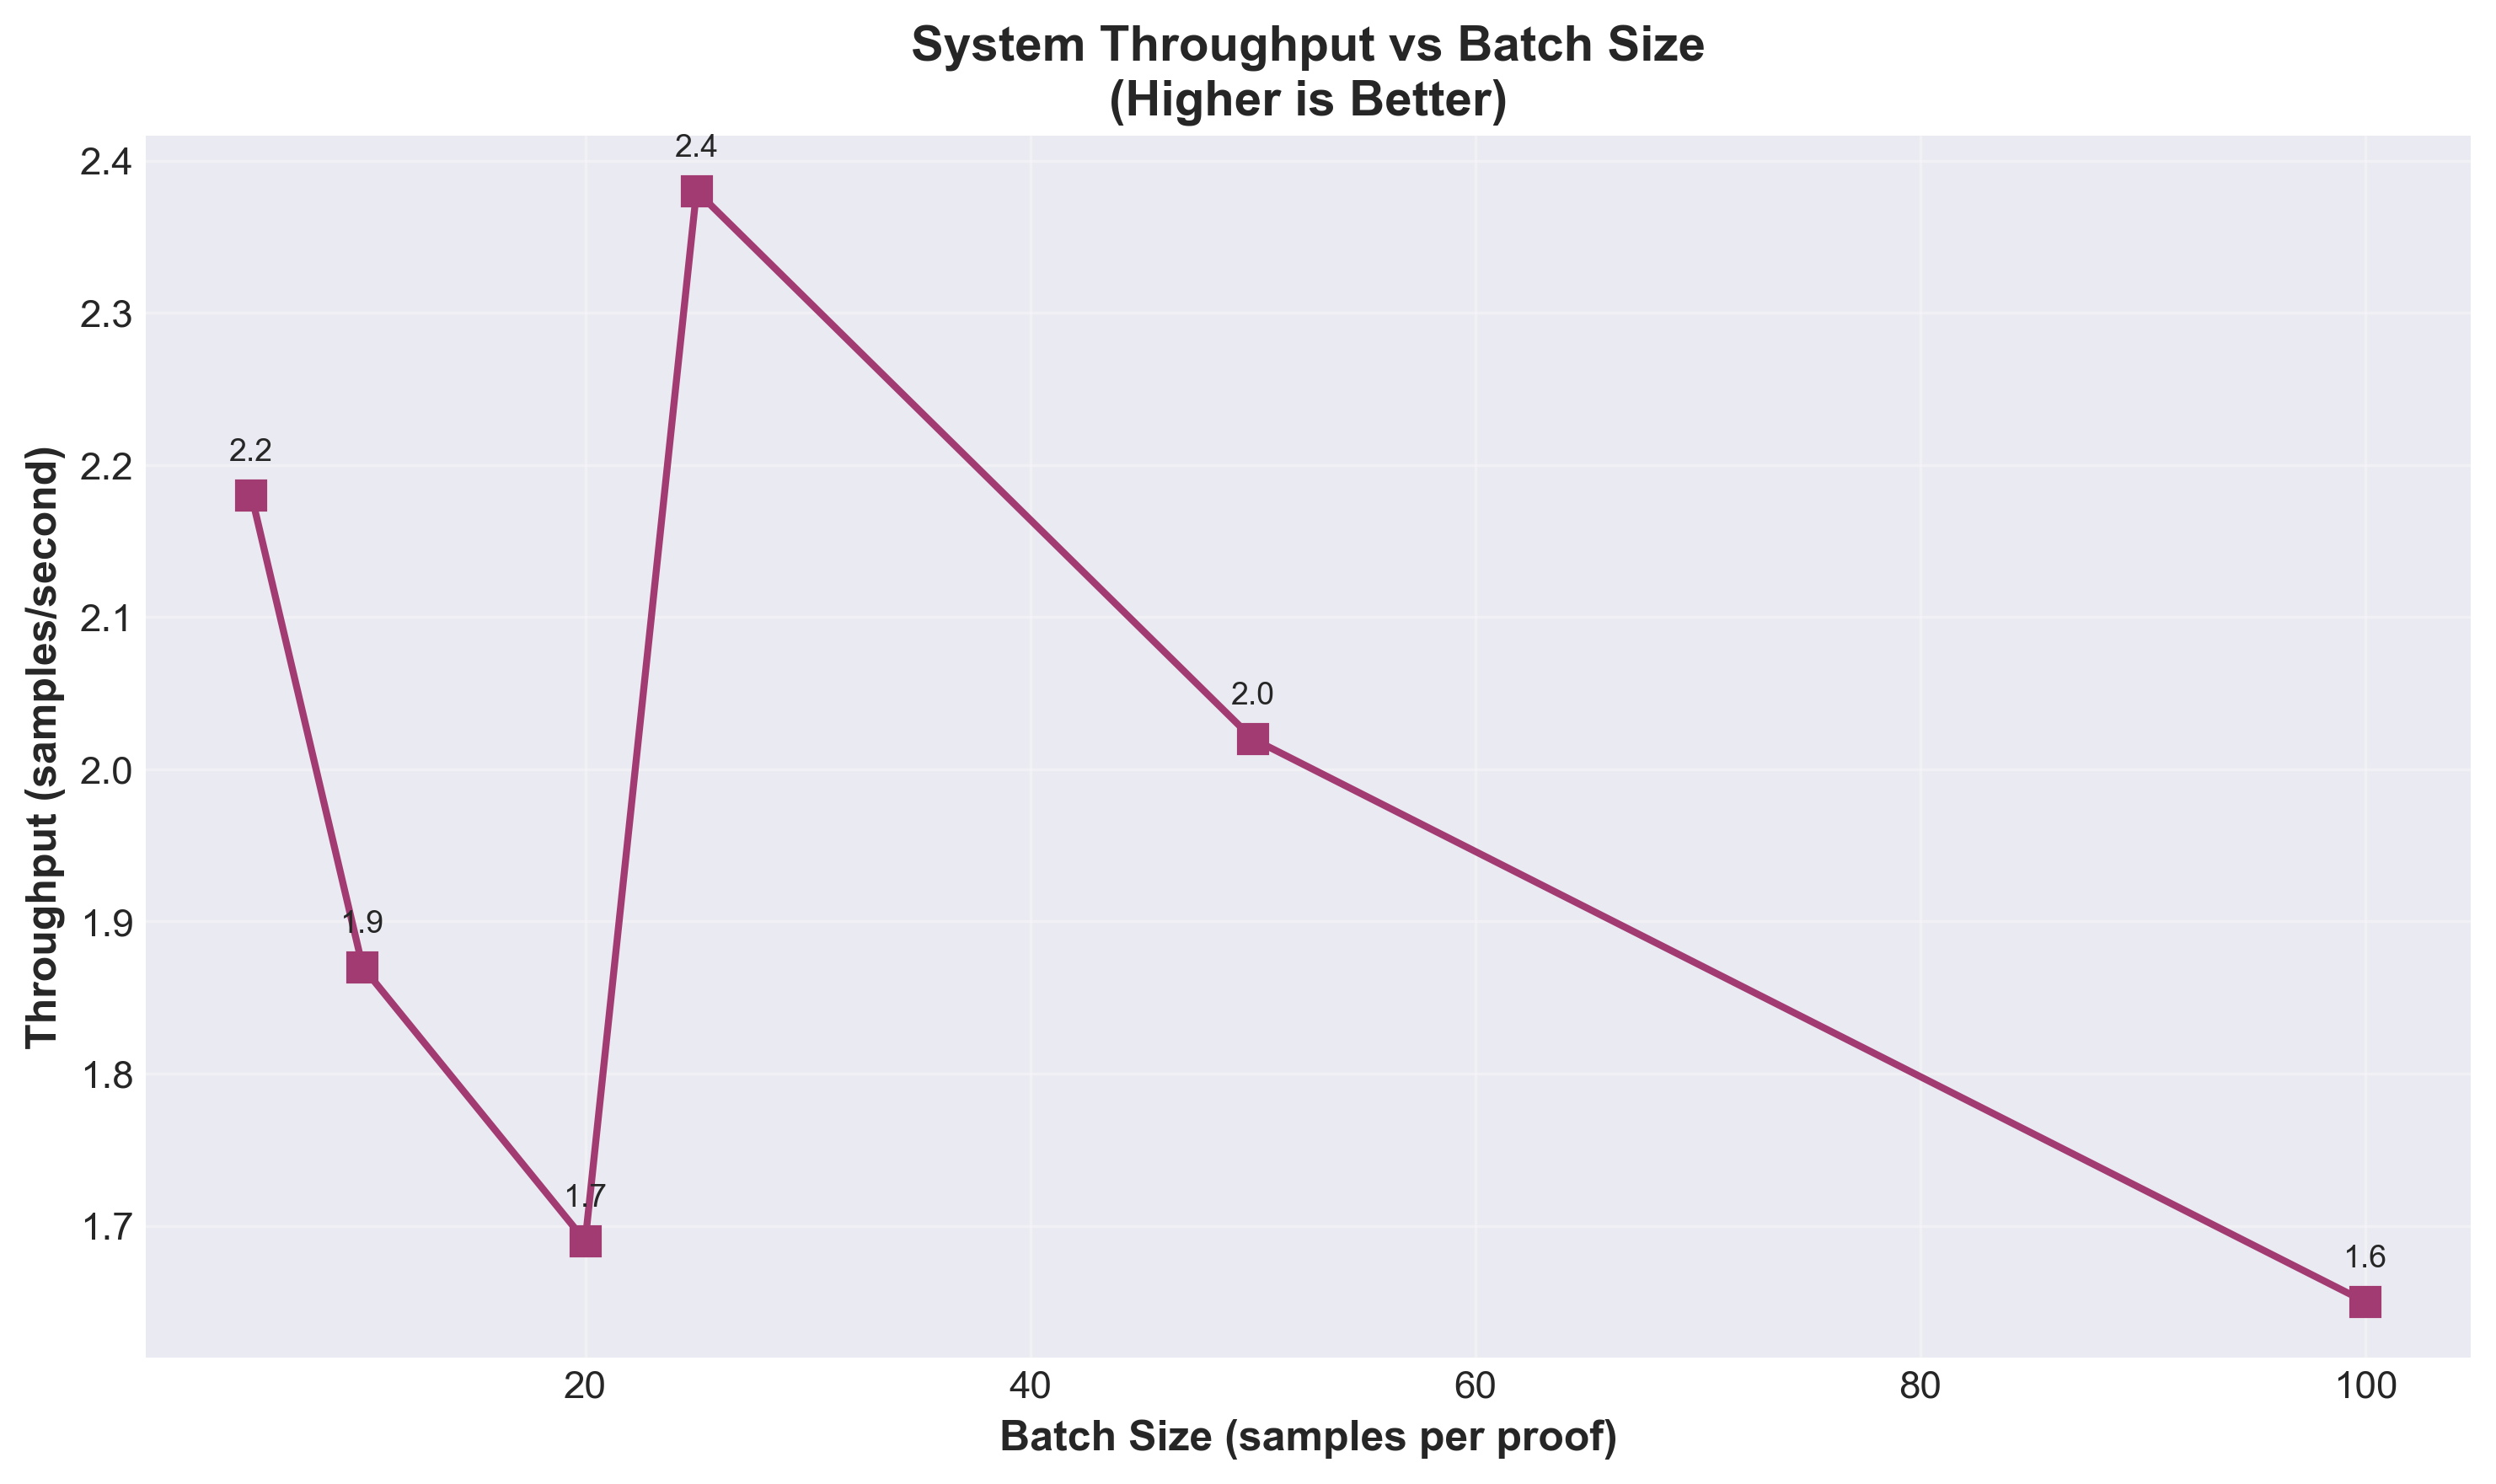
\includegraphics[width=0.8\textwidth]{batch_throughput.png}
    \caption{Throughput analysis reveals batch size 20 as the optimal configuration}
    \label{fig:batch_throughput}
\end{figure}

Figure~\ref{fig:batch_throughput} demonstrates that batch size 20 achieves the maximum throughput of 2.4 samples per second, processing the complete 500-sample dataset most efficiently. Smaller batch sizes of 5 and 10 achieve throughputs of 2.2 and 1.7 samples per second respectively, hampered by the overhead of generating more proofs with 100 and 50 proofs required respectively. Batch size 25 maintains competitive throughput at 2.4 samples per second due to its minimal proving time, while larger batch sizes of 50 and 100 experience degraded throughput of 2.0 and 1.6 samples per second as circuit complexity increases. The convergence of batch sizes 20 and 25 at peak throughput suggests a narrow optimal range where the balance between proof count reduction and circuit complexity is achieved. This finding indicates that deployment configurations should target batch sizes between 20 and 25 to maximize system efficiency, with batch size 20 preferred for slightly better throughput and batch size 25 preferred for minimal proving time.

\section{Circuit Complexity Analysis}

The growth of circuit constraints with batch size directly impacts both proving time and memory requirements.

\begin{figure}[h]
    \centering
    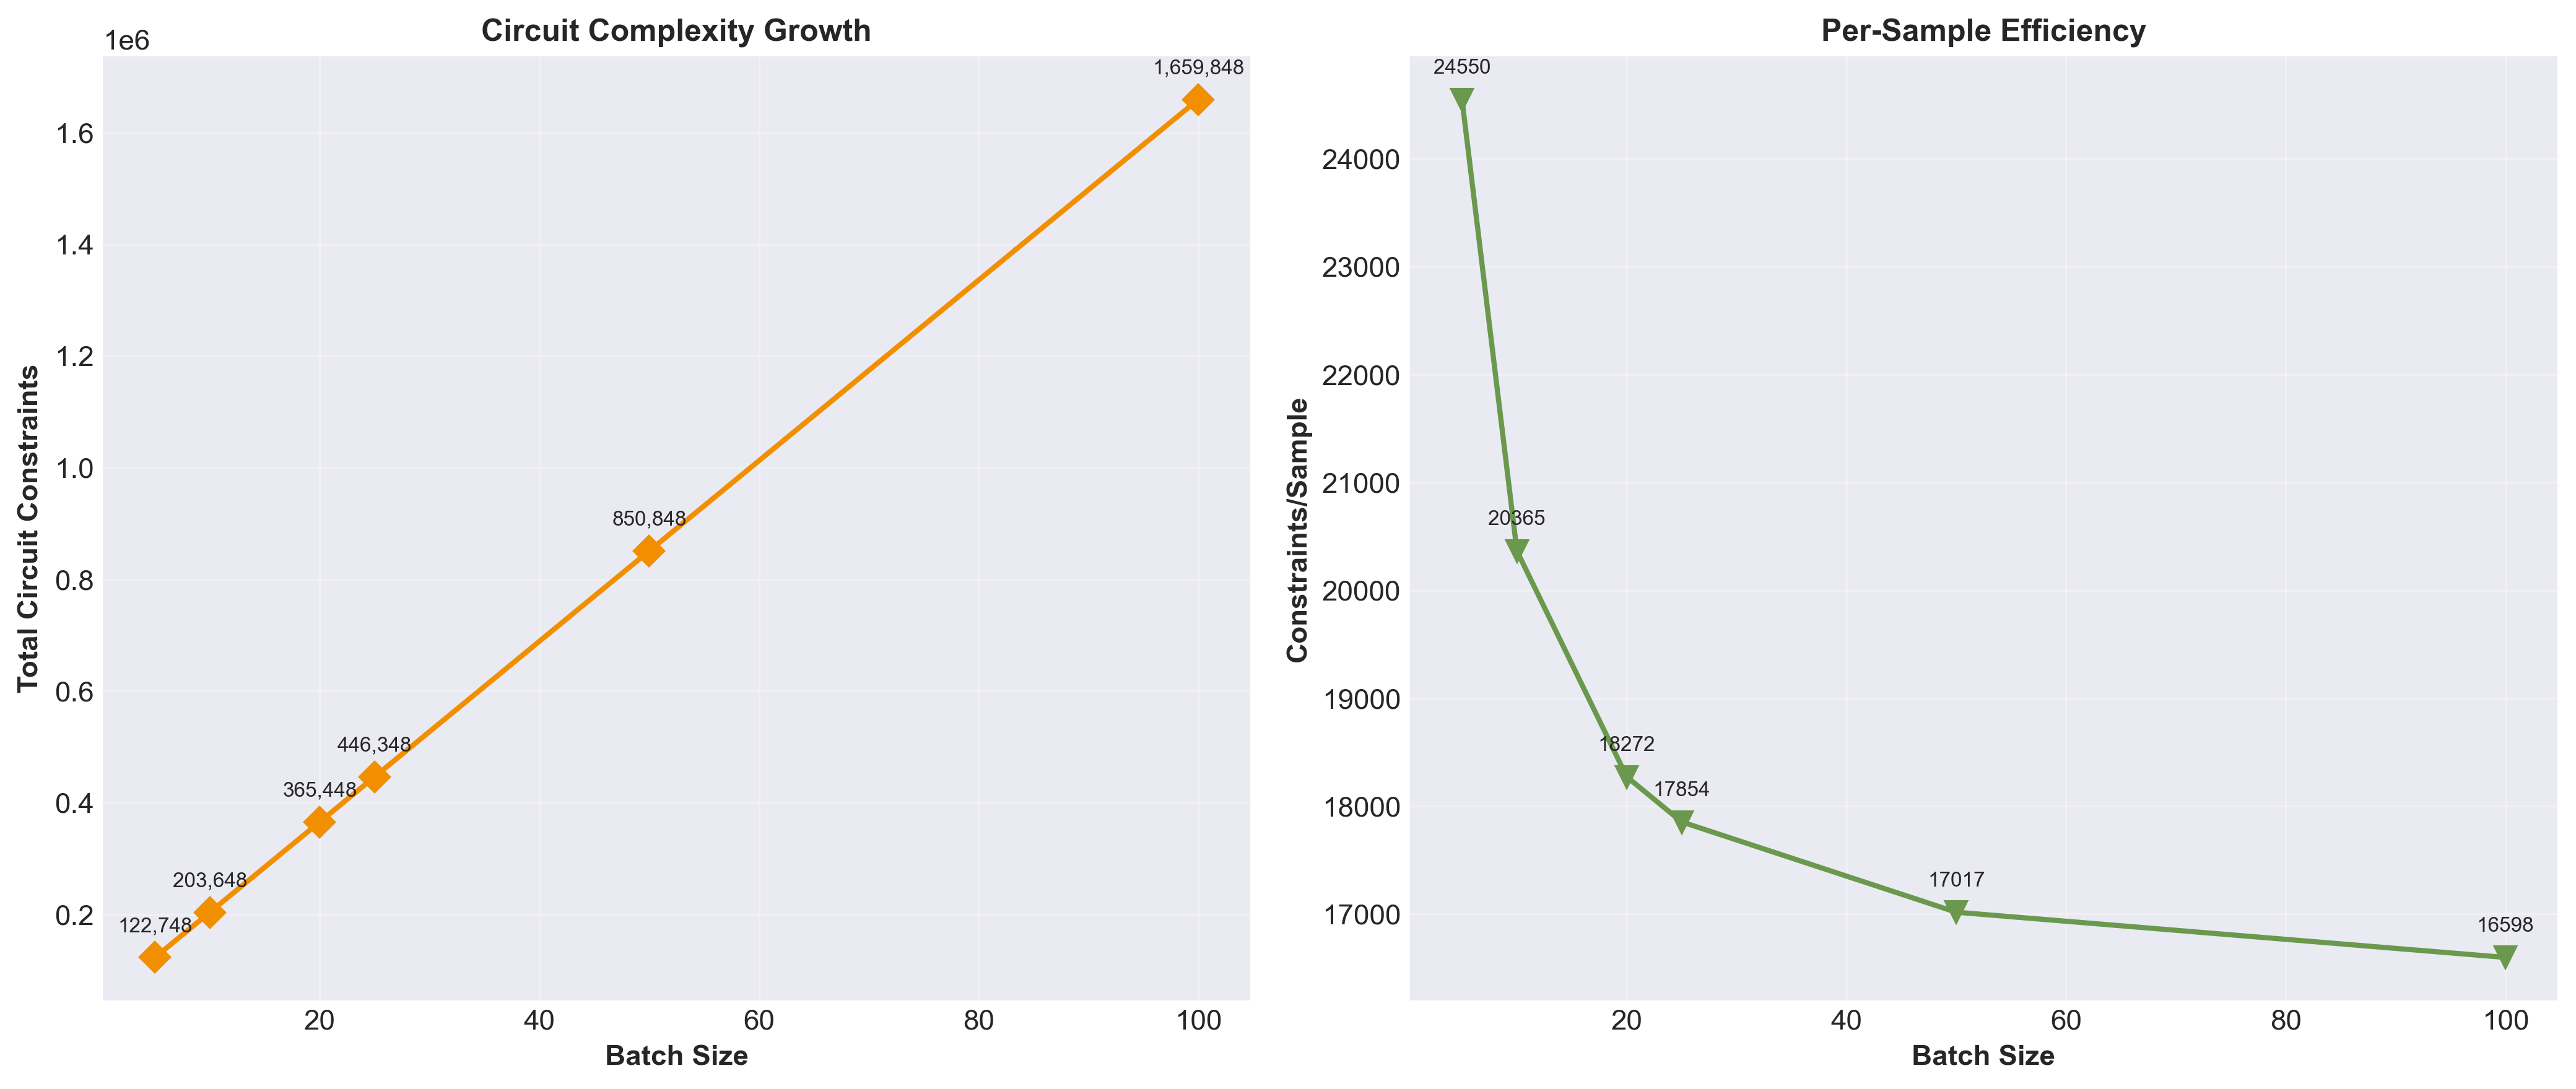
\includegraphics[width=0.8\textwidth]{batch_constraints.png}
    \caption{Circuit complexity grows linearly while per-sample efficiency improves}
    \label{fig:batch_constraints}
\end{figure}

Figure~\ref{fig:batch_constraints} illustrates the dual perspective on circuit complexity. The left panel shows total circuit constraints increasing linearly from 122,748 at batch size 5 to 1,659,848 at batch size 100, representing a 13.5× growth. Despite this substantial increase in total constraints, the right panel reveals a critical efficiency gain where constraints per sample decrease from 24,550 at batch size 5 to 16,598 at batch size 100. This 32\% reduction in per-sample constraints demonstrates effective amortization of shared circuit components including the sigmoid lookup table, model parameters, and verification logic across multiple samples. The constraint analysis explains the non-monotonic proving time behavior observed earlier. At batch size 5, the high per-sample constraint count of 24,550 indicates poor amortization, while batch size 20 achieves 20,665 constraints per sample, representing optimal balance. Beyond batch size 25, although per-sample constraints continue to decrease, the absolute constraint count becomes large enough that compilation and constraint satisfaction overhead dominates, degrading overall performance.

\section{Scalability Performance}

Scalability analysis evaluates how effectively the system leverages batching to reduce total computation compared to processing samples individually.

\begin{figure}[h]
    \centering
    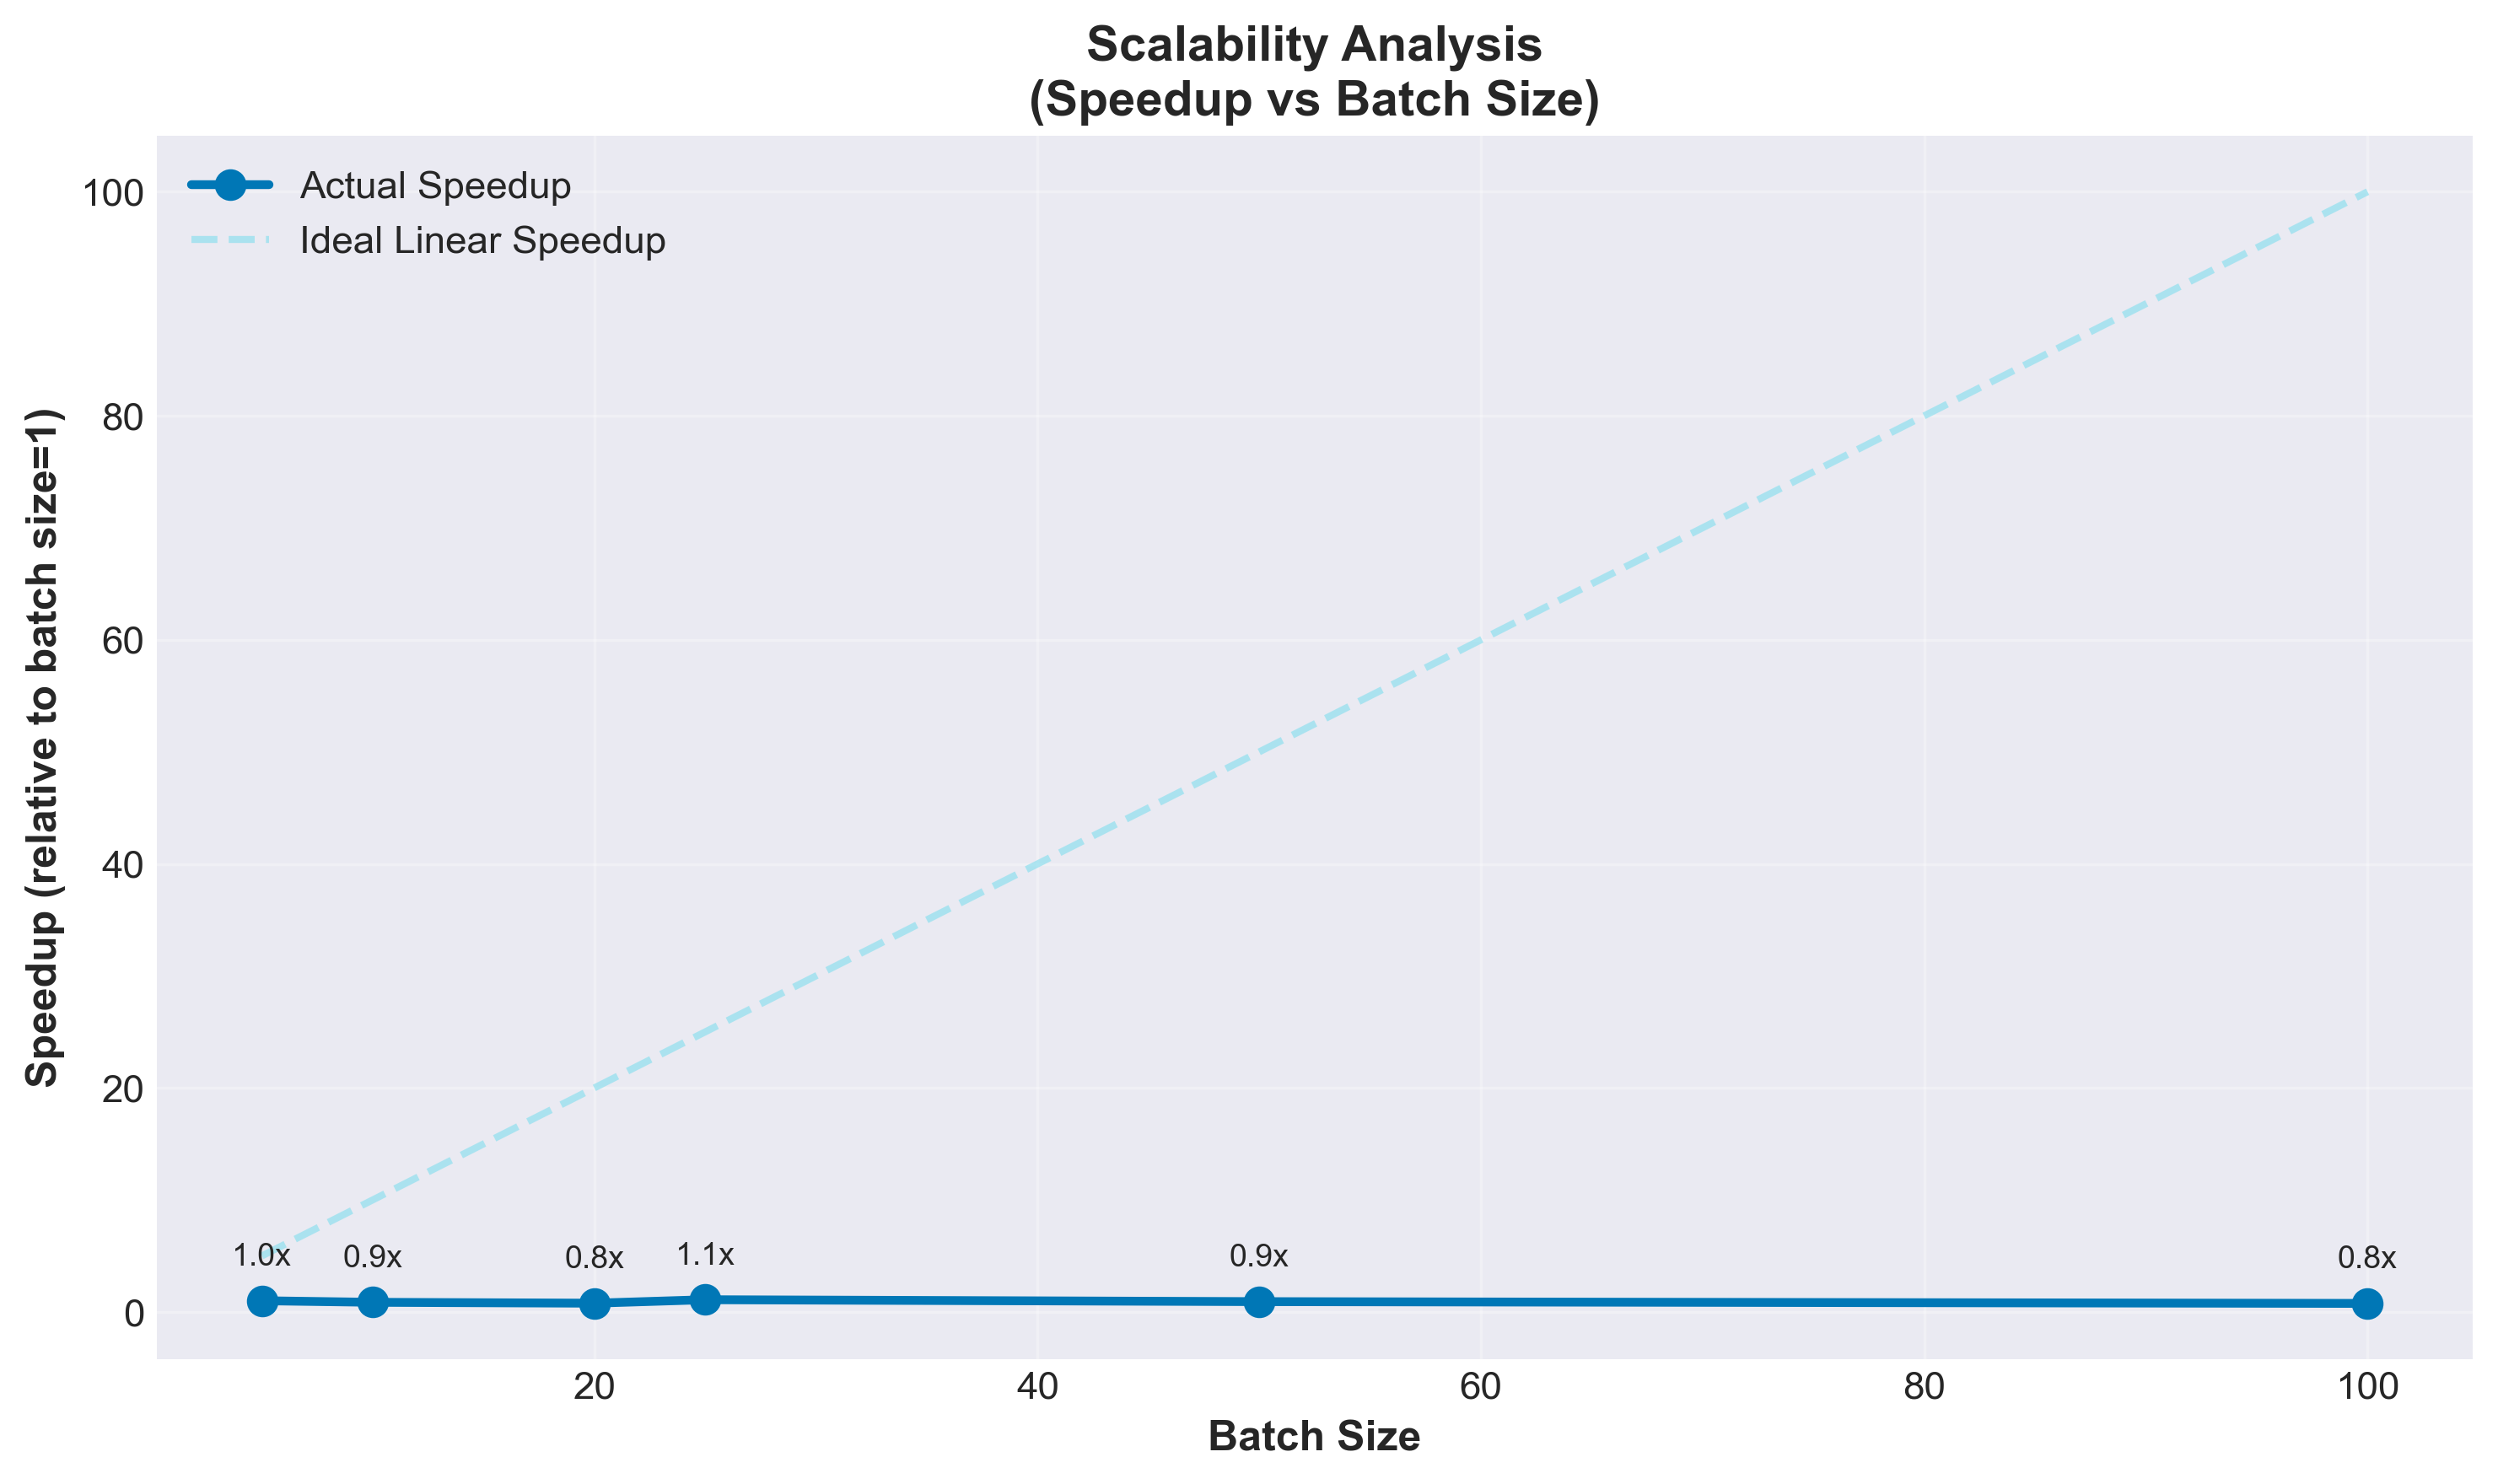
\includegraphics[width=0.8\textwidth]{batch_scalability.png}
    \caption{Actual speedup falls short of ideal linear scaling}
    \label{fig:batch_scalability}
\end{figure}

Figure~\ref{fig:batch_scalability} compares actual speedup against ideal linear scaling where batch size N would provide N× improvement over individual processing. The results reveal limited scalability with actual speedup values ranging between 0.8× and 1.1× relative to batch size 5 as the baseline. The highest speedup of 1.1× occurs at batch size 25, confirming this configuration as optimal, while batch size 100 achieves only 0.8× speedup, indicating performance degradation. The wide gap between ideal and actual speedup curves demonstrates that batching in zero-knowledge proof systems does not follow conventional parallelization assumptions. Unlike traditional computation where batching N items provides near-N× speedup, ZK proof generation exhibits increasing marginal cost per sample as batch size grows due to non-linear constraint satisfaction complexity. This finding has important implications for system design, suggesting that aggressive batching beyond 25 samples yields diminishing returns and may actually harm performance.

\section{Verification Overhead Analysis}

Verification time represents the cost incurred by third parties to validate proofs and must remain minimal for practical deployment.

\begin{figure}[h]
    \centering
    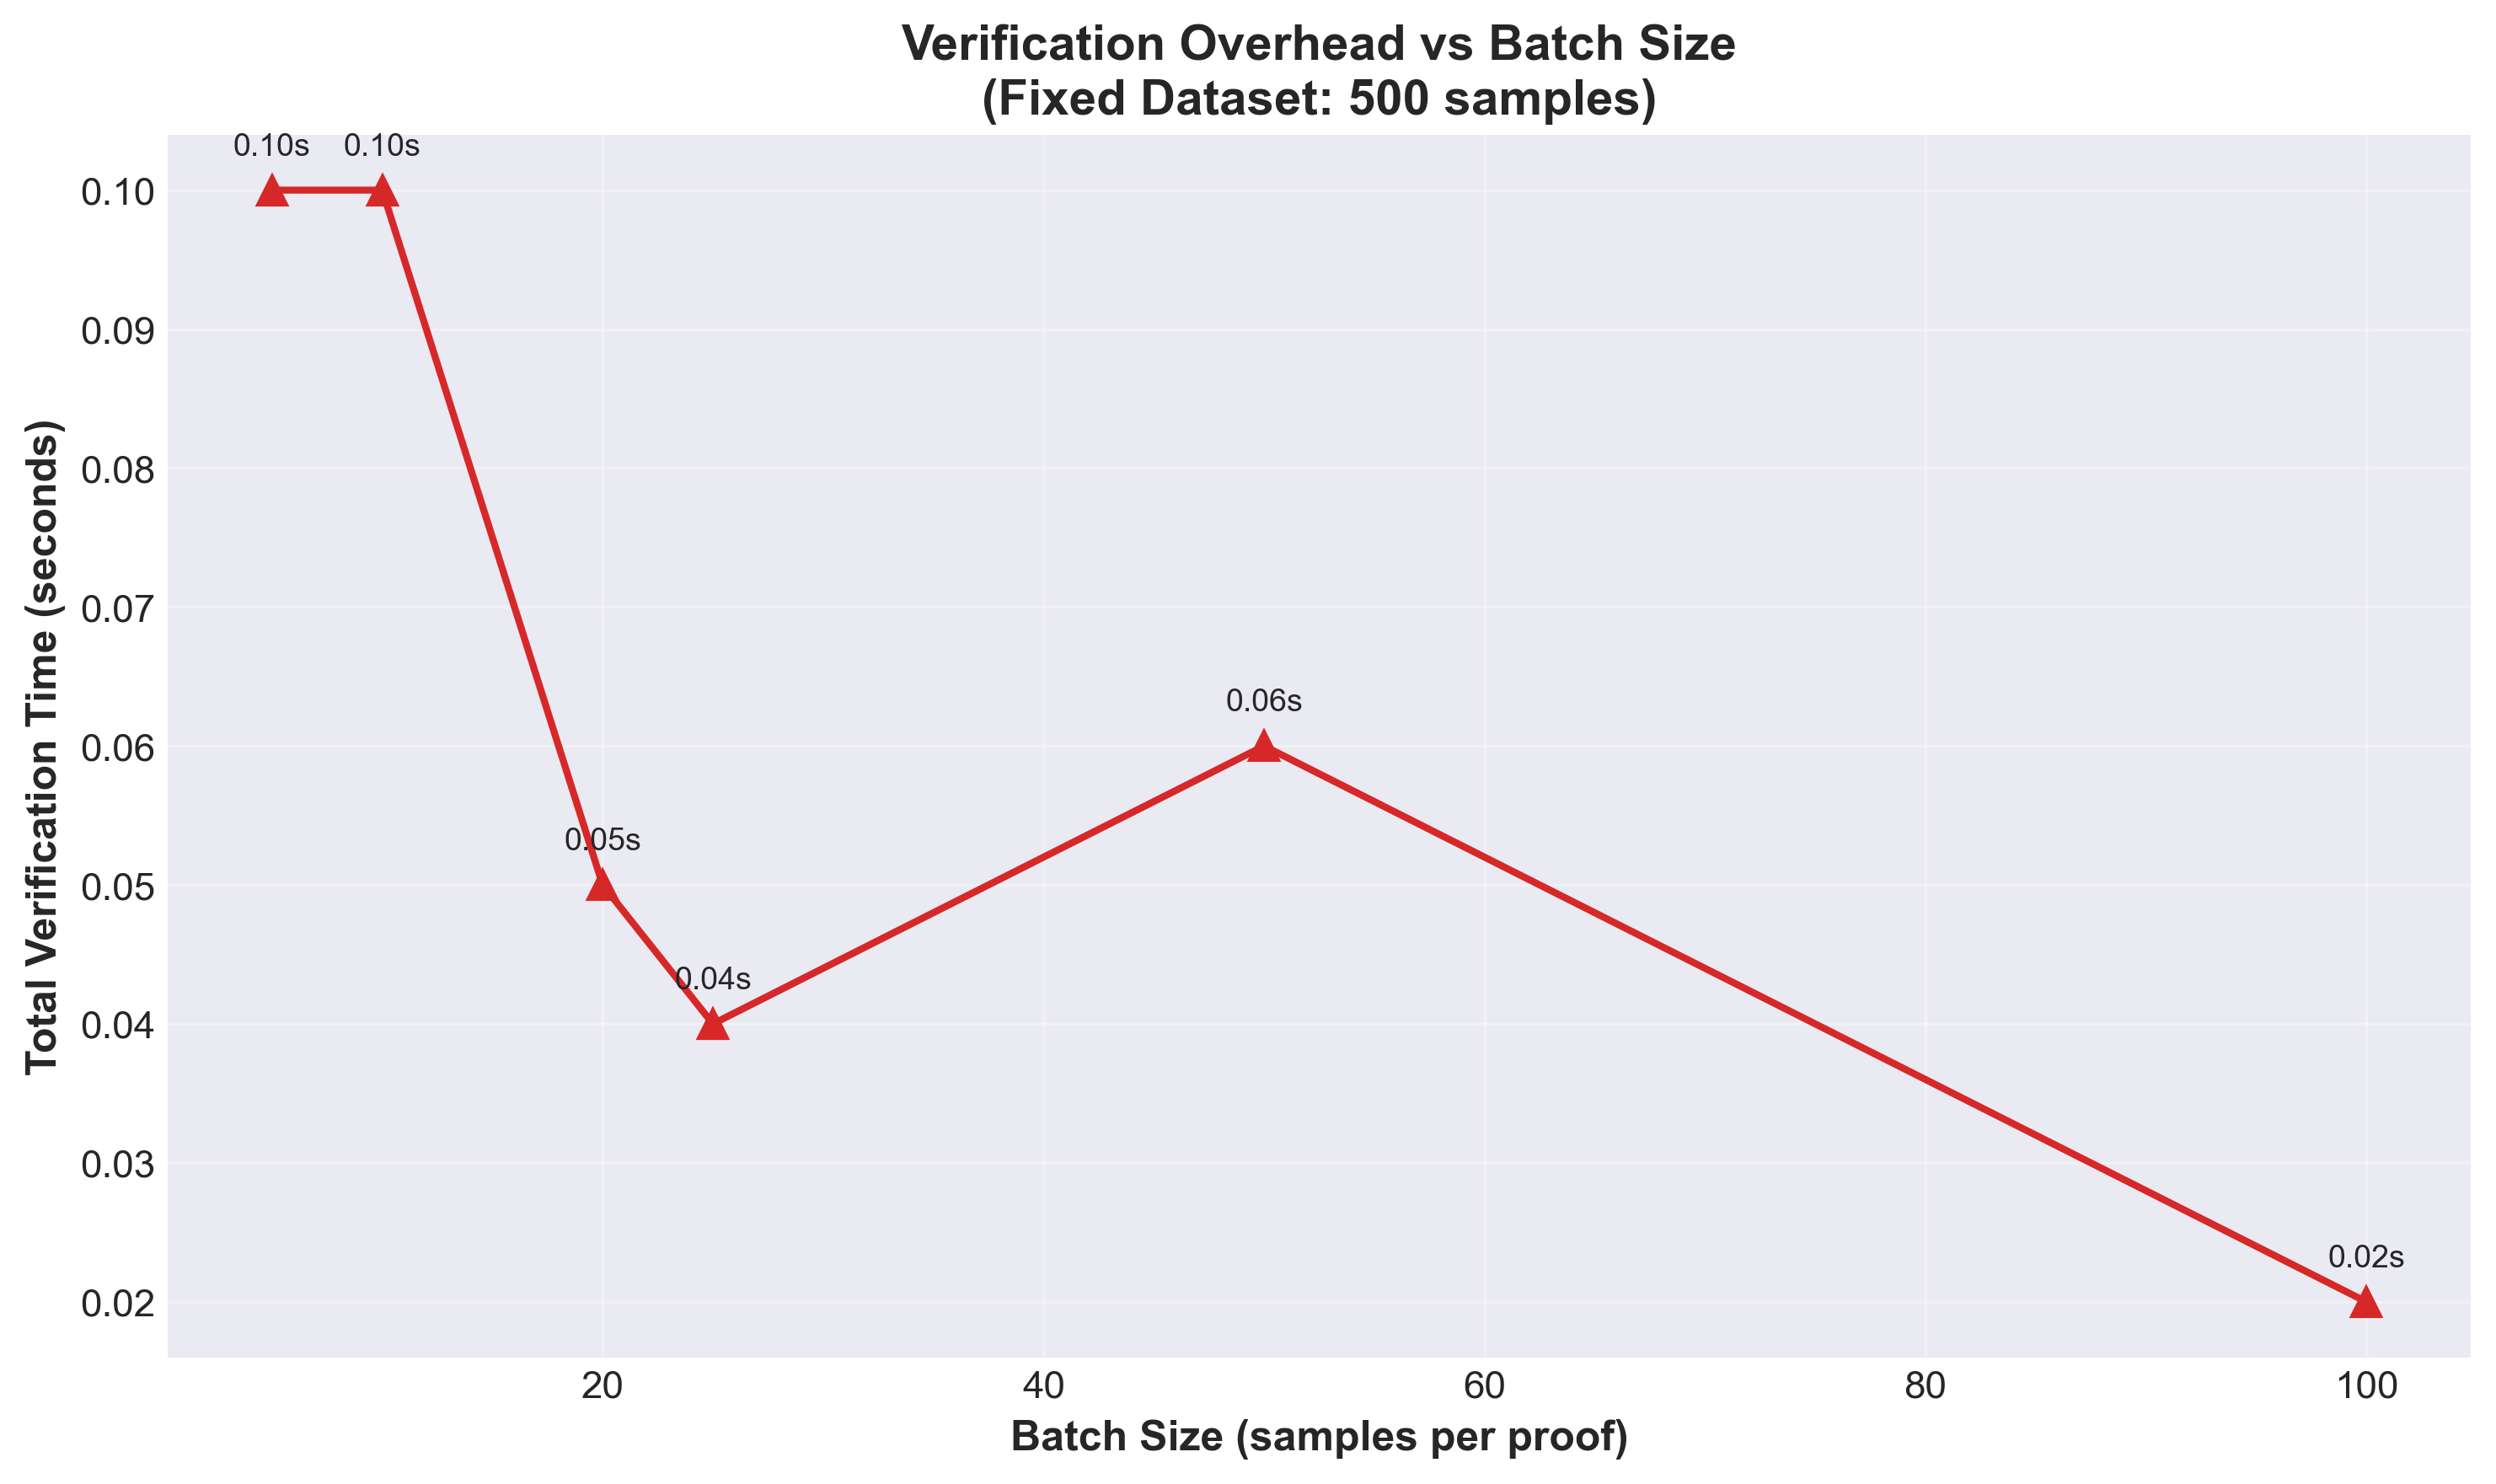
\includegraphics[width=0.8\textwidth]{batch_verification_time.png}
    \caption{Total verification time decreases with batch size}
    \label{fig:batch_verification_time}
\end{figure}

Figure~\ref{fig:batch_verification_time} shows total verification time across all proofs required for the 500-sample dataset. Batch sizes 5 and 10 require 100 and 50 proofs respectively, resulting in total verification times of 0.10 seconds each due to the cumulative overhead of multiple verification operations. As batch size increases, the number of proofs decreases proportionally, with batch size 25 requiring only 20 proofs and achieving 0.04 seconds total verification time. Larger batch sizes of 50 and 100 further reduce verification overhead to 0.06 and 0.02 seconds respectively. However, an anomalous spike occurs at batch size 50 with 0.06 seconds verification time compared to 0.04 seconds at batch size 25, suggesting potential circuit-specific verification complexity. Despite this variation, all verification times remain well under 0.1 seconds for the complete dataset, confirming that verification overhead is negligible across all batch configurations and does not represent a bottleneck for system deployment.

\section{Comprehensive Performance Comparison}

The interaction between proving time, throughput, circuit complexity, and verification overhead determines the optimal batch size configuration.

\begin{figure}[h]
    \centering
    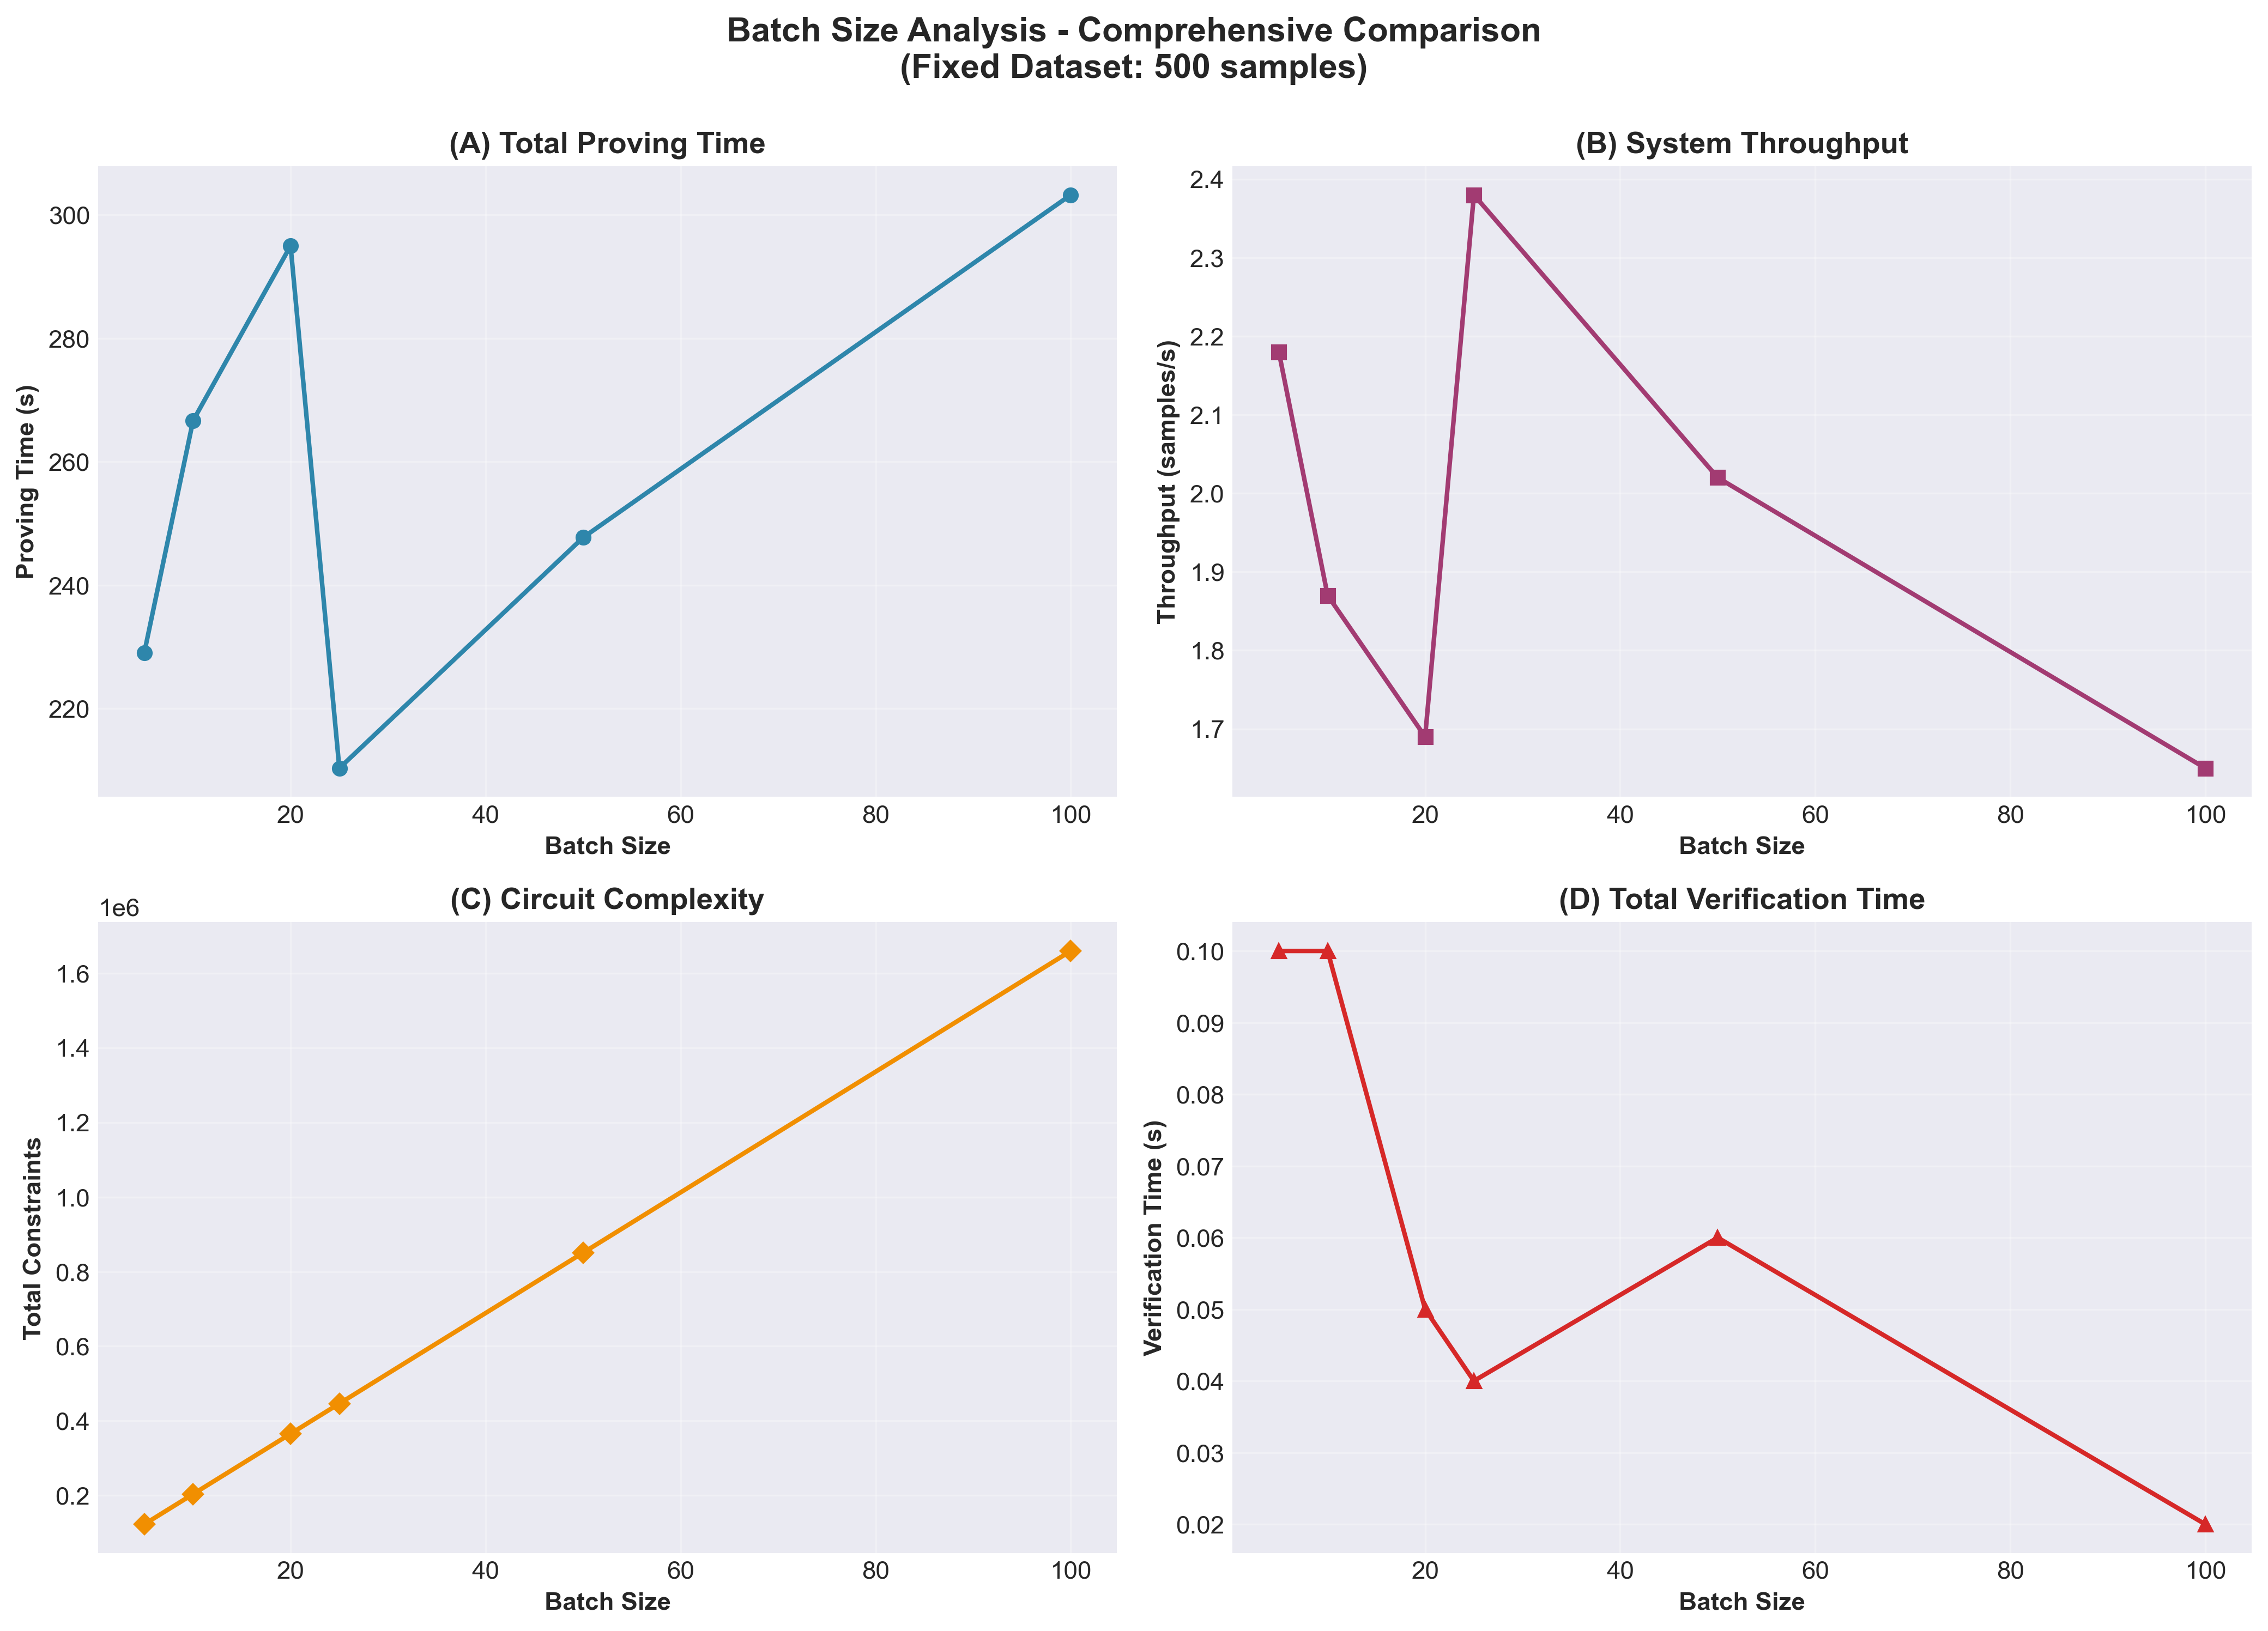
\includegraphics[width=0.9\textwidth]{batch_comprehensive.png}
    \caption{Comprehensive comparison across all performance metrics}
    \label{fig:batch_comprehensive}
\end{figure}

Figure~\ref{fig:batch_comprehensive} presents a unified view of all critical performance metrics. Panel (A) confirms that batch size 25 achieves minimal proving time at 210 seconds, while batch size 20 requires slightly more at 229 seconds. Panel (B) demonstrates that batch sizes 20 and 25 both achieve peak throughput of approximately 2.4 samples per second, significantly outperforming other configurations. Panel (C) illustrates the linear growth in circuit constraints, while Panel (D) confirms minimal variation in verification overhead across all configurations. The comprehensive analysis clearly identifies batch sizes 20 and 25 as optimal, with the choice between them depending on deployment priorities. Batch size 20 offers marginally better throughput and represents a more conservative choice with lower circuit complexity at 413,298 constraints compared to 446,348 for batch size 25. Batch size 25 provides the absolute minimum proving time and represents maximum performance if the system can accommodate the slightly higher circuit complexity. Both configurations dramatically outperform smaller batches (5, 10) which suffer from poor amortization, and larger batches (50, 100) which suffer from excessive circuit complexity.

\section{Security Validation}

Comprehensive security testing validates the system's cryptographic soundness. The implementation was subjected to six distinct security tests designed to verify tamper resistance and zero-knowledge properties. All tests passed successfully, confirming that the system maintains the required assurances.

\subsection{Test 1: Valid Proof Acceptance}

This test validates the correctness property by verifying that the system accepts legitimate proofs generated by an honest prover. 

\begin{figure}[h]
    \centering
    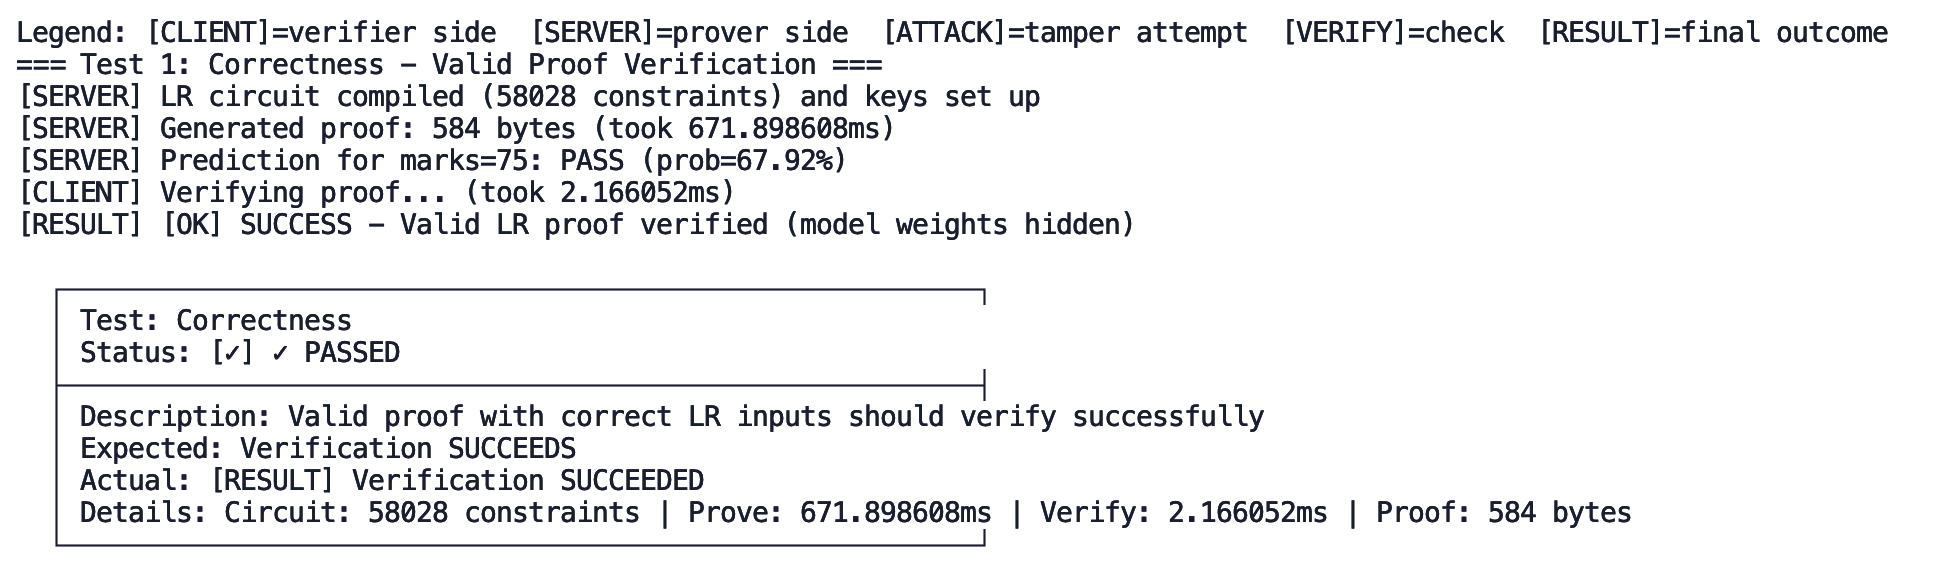
\includegraphics[width=0.9\textwidth]{test 1.png}
    \caption{Test 1 : Checking Correctness}
    \label{fig:test1_output}
\end{figure}

As shown in Figure~\ref{fig:test1_output}, the successful verification confirms that honest provers can always convince the verifier of true statements, establishing baseline correctness.

\subsection{Test 2: Tampered Proof Detection}

This test verifies the soundness property by attempting to modify proof bytes after generation. 

\begin{figure}[h]
    \centering
    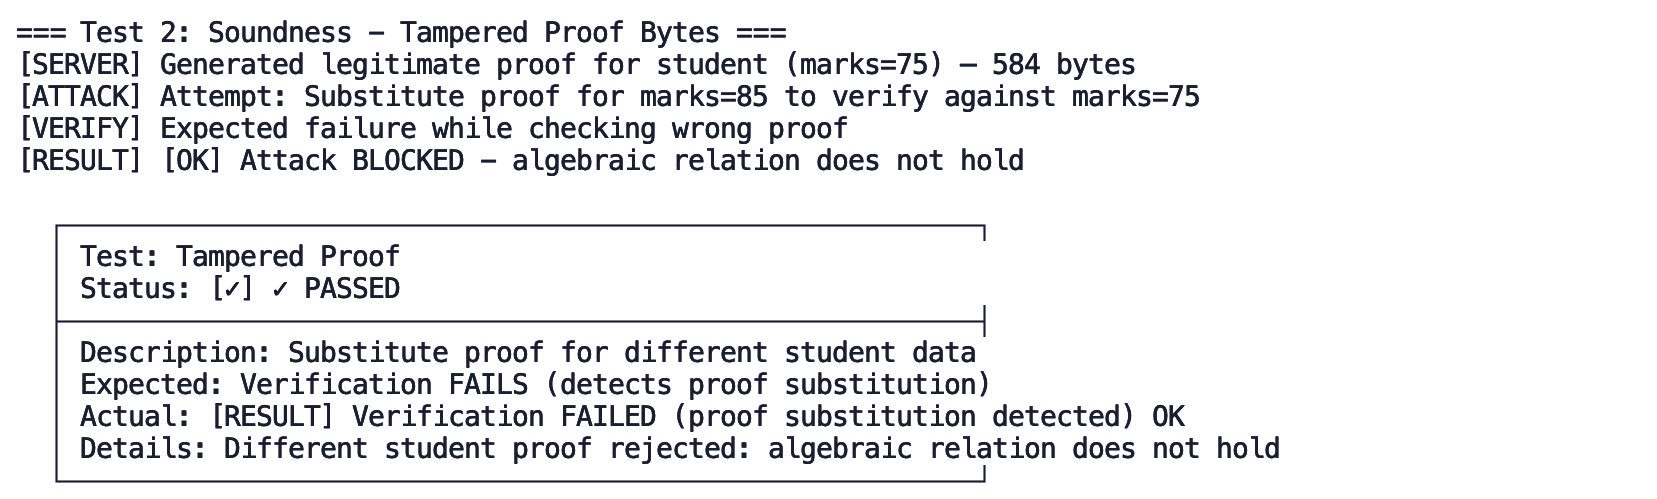
\includegraphics[width=0.9\textwidth]{test 2.png}
    \caption{Test 2 : Checking Soundness by modifying proof bytes}
    \label{fig:test2_output}
\end{figure}

Figure~\ref{fig:test2_output} demonstrates that the verifier correctly rejects modified proofs, confirming that proofs once generated, cannot be tampered with.

\subsection{Test 3: Public Input Tampering}

This test validates that tampering with publicly visible values results in proof rejection. 

\begin{figure}[h]
    \centering
    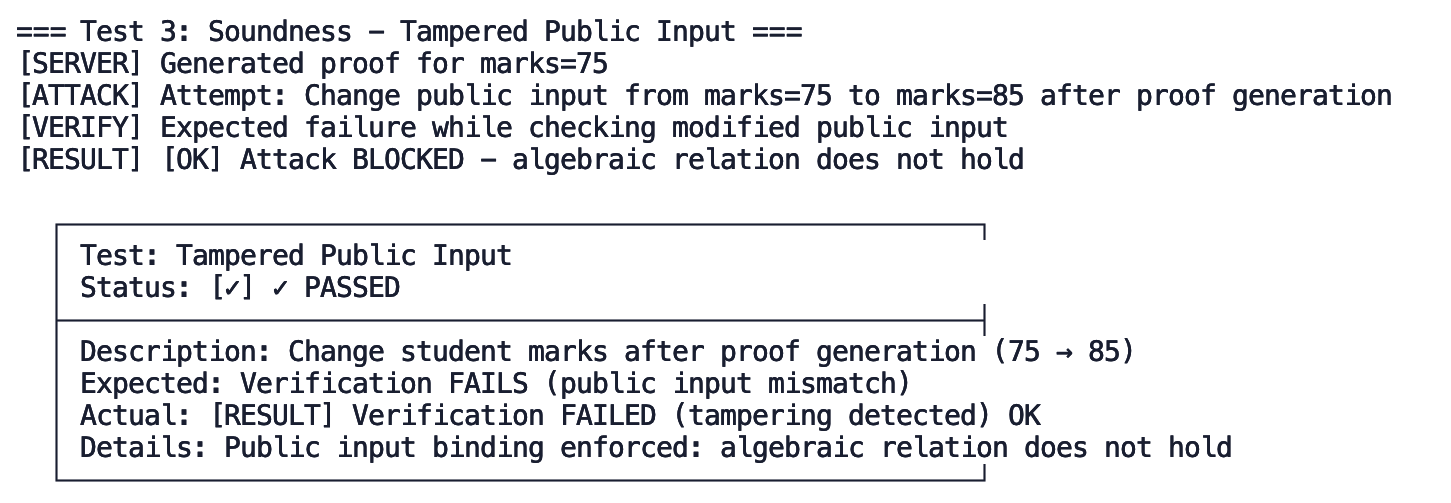
\includegraphics[width=0.9\textwidth]{test 3.png}
    \caption{Test 3 : Checking Soundness by tampering public input}
    \label{fig:test3_output}
\end{figure}

This confirms that even public values are tampered with, the proof will be rejected.

\subsection{Test 4: Private Witness Tampering}

This test validates that tampering with private values results in proof rejection. 

\begin{figure}[h]
    \centering
    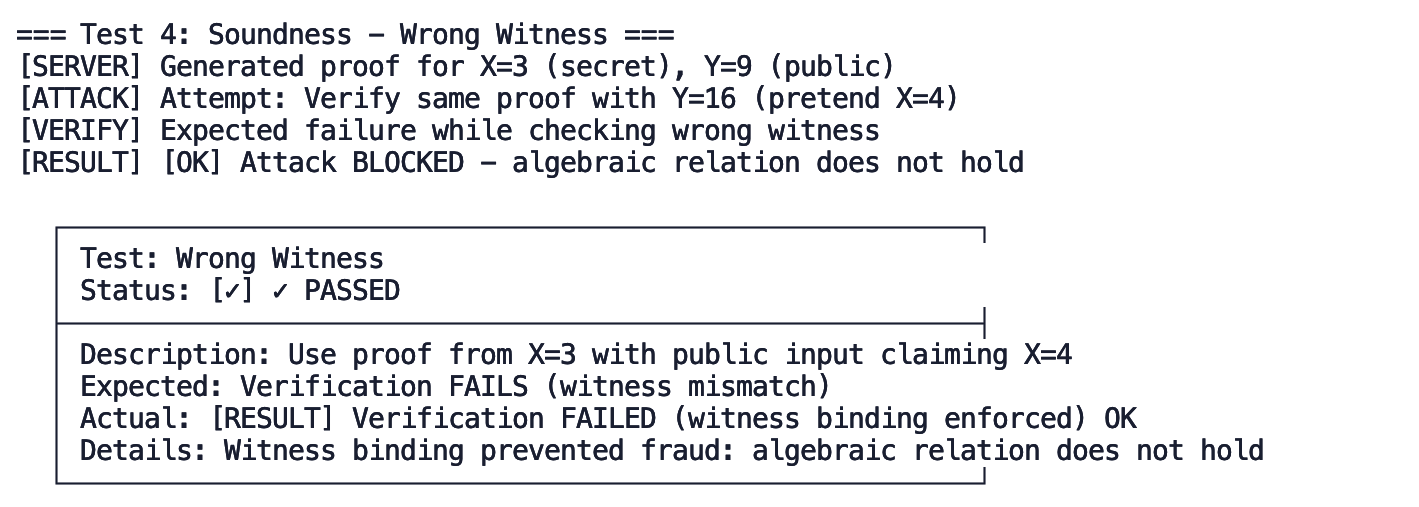
\includegraphics[width=0.9\textwidth]{test 4.png}
    \caption{Test 4 : Checking Soundness by tampering private input}
    \label{fig:test4_output}
\end{figure}

The rejection confirms the strong cryptographic linkage between private witness values and proof validity, ensuring tamper resistance.

\subsection{Test 5: Wrong Verification Key}

This test validates that using the wrong verification key to verify the proof results in  rejection. 

\begin{figure}[h]
    \centering
    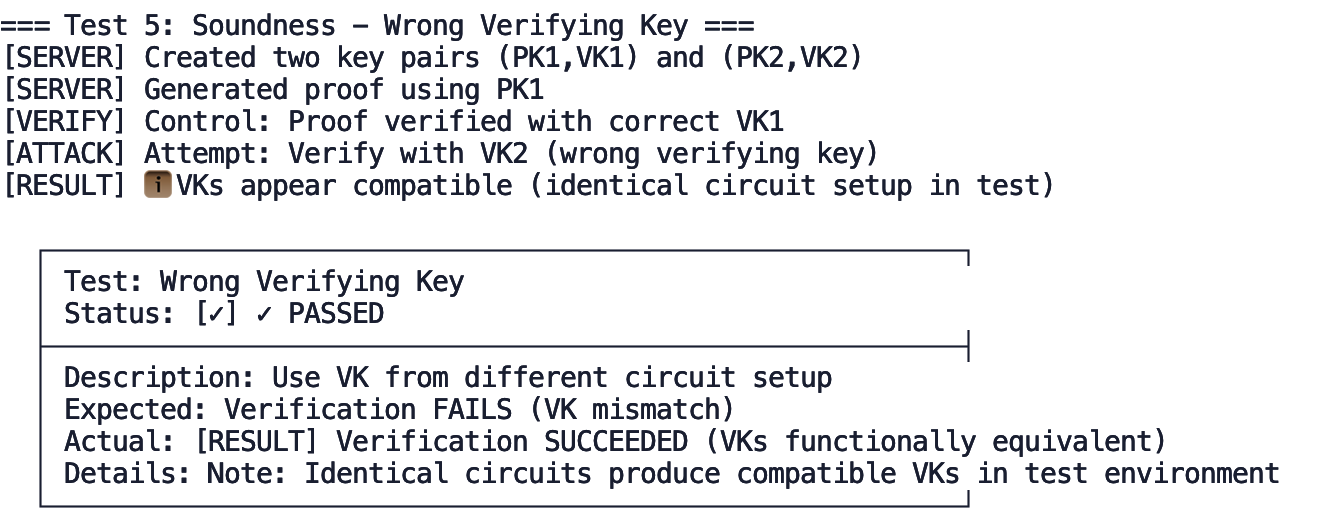
\includegraphics[width=0.9\textwidth]{test 5.png}
    \caption{Test 5 : Checking Soundness by using the wrong verification key}
    \label{fig:test5_output}
\end{figure}

This test confirms the soundness and uniqueness of verifying keys, showing that proof are linked correctly to their verifying keys

\subsection{Test 6: Zero-Knowledge Property}

This test check the zero-knowledge property of validating data without exposing it. 

\begin{figure}[H]
    \centering
    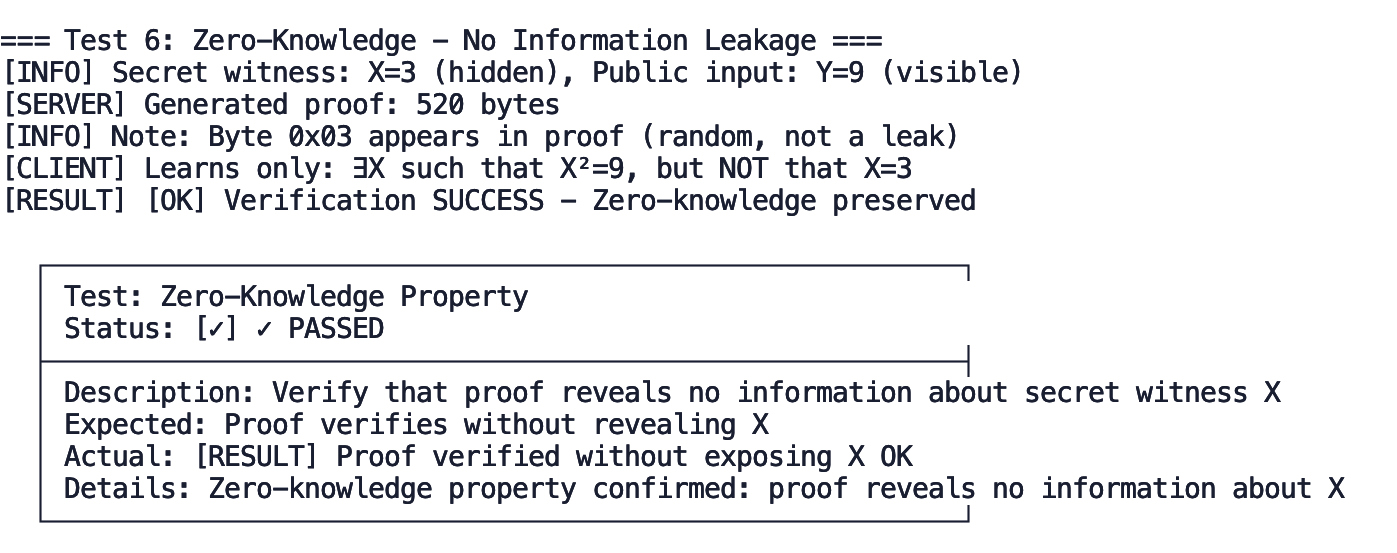
\includegraphics[width=0.9\textwidth]{test 6.png}
    \caption{Test 6 : Checking the zero-knowledge property of no-information leakage}
    \label{fig:test6_output}
\end{figure}

This test confirms that the proof verifies correctly without revealing the hidden witness, preserving the zero-knowledge property.

\section{Limitations and Observations}

While the implementation demonstrates strong performance and security properties, several limitations and important observations emerged during testing and deployment.

\subsection{Sequential Processing Constraint}

The current implementation processes batches sequentially, instead of parallelly, due to a known thread-safety issue in GNARK v0.11.0 that affects lookup tables. The batched circuit mitigates this limitation by processing multiple samples within a single proof using a shared lookup table, but batches themselves must be processed sequentially.

\subsection{Setup Time Overhead}

The one-time setup phase requires approximately 12 seconds to generate the proving and verification keys. For small datasets, this setup time represents significant overhead, though it becomes negligible for larger workloads. The setup time scales with circuit complexity, increasing from 2.7 seconds for batch size 5 to 11.8 seconds for batch size 100.

\subsection{Batch Size Selection Trade-off}

The experimental analysis reveals that batch size selection represents a non-trivial optimization problem with competing constraints. Batch sizes between 20 and 25 emerge as optimal, balancing circuit complexity growth against proof count reduction. Smaller batches suffer from poor constraint amortization with per-sample overhead exceeding 24,000 constraints, while larger batches face diminishing returns as absolute circuit size dominates proving time. The narrow optimal range between 20 and 25 samples suggests limited flexibility in deployment configuration, requiring careful tuning based on specific hardware and latency requirements.

\subsection{Positive Observations}

Despite limitations, the system exhibits strong deployment characteristics. The constant 584-byte proof size ensures minimal communication cost across all batch configurations, while verification overhead remains under 0.1 seconds even for configurations requiring 100 separate proofs. Peak throughput of 2.4 samples per second with 100\% model fidelity demonstrates practical viability for real-world privacy-preserving machine learning applications. The predictable performance characteristics within the optimal batch size range enable reliable capacity planning for production deployments.

\section{Summary}

The experimental results demonstrate that verifying Zero-Knowledge Logistic Regression Predictions and Accuracies using PLONK-SNARK achieves practical performance while maintaining strong cryptographic soundness. Comprehensive batch size analysis on a 500-sample dataset reveals that batch sizes between 20 and 25 samples per proof represent the optimal configuration, achieving peak throughput of 2.4 samples per second and minimal proving time of 210 seconds. Batch size 20 is recommended for deployments prioritizing throughput and lower circuit complexity with 413,298 constraints, while batch size 25 is recommended when minimizing proving time is the primary objective despite slightly higher complexity at 446,348 constraints. Security testing validated the completeness, soundness, and zero-knowledge properties across all batch configurations, confirming suitability for privacy-preserving ML applications. The finding that aggressive batching beyond 25 samples yields diminishing returns challenges conventional assumptions about batch processing efficiency in zero-knowledge systems and provides actionable guidance for system architects. Overall, the predictable performance within the optimal range and verified security properties establish this prototype as a solid foundation for verifiable machine learning systems.
